\documentclass{tufte-handout}

\usepackage{style}

\begin{document}

\tma{03} % TMA number

\section{Part A}

%Question 1
\begin{question}

\qpart

\[ 1573 = 11^{2} \times 13 \]

Using \textup{Proposition 2.3, HB chapter 2 p17};

for \( n \geq 2 \), \( n = p_{1}^{k_1}p_{2}^{k_2}\ldots p_{r}^{k_r} \), then

\[ \tau(n) = (k_{1}+1)(k_{2}+1)\ldots (k_{r}+1) = 1573 = 11^{2} \times 13 \]

Where \( \tau(n) \) is the number of positive divisors of \( n \).

\begin{align*}
k_{1}+1 = 13 &\implies k_{1} = 12 \\[8pt]
k_{2}+1 = 11 &\implies k_{2} = 10 \\[8pt]
k_{3}+1 = 11 &\implies k_{3} = 10 \\[8pt]
\end{align*}

Any other allocation either increases the largest exponent or introduces larger primes, producing a larger integer.

To minimise \( n \), we assign the largest exponent to the smallest prime, the second largest exponent to the 
second smallest prime, and so on.

Since \( 1573 = 13 \cdot 11 \cdot 11, \text{ we choose exponents } 12,10,10 \)

Hence the smallest positive integer \( n \) with exactly \( 1573 \) positive divisors is
\[ \boxed{ n = 2^{12} \cdot 3^{10} \cdot 5^{10} } \]



\vspace{3cm}

\qpart

Let \( n \) be the positive integer such that
\[ 7n + \sigma(n) \mid 8 \]

Where \( \sigma(n) \) is the sum of divisors function.

If \( n = p^{2} \) (where \( p \) is prime), then \( p \equiv 7 \pmod{8} \)

\begin{proof}

$$ \newline

The divisors of \( p^{2} \) are \( 1, p \text{ and } p^{2} \)

Using \textup{Proposition 1.2, HB Chapter 9 p48};

\[ \sigma(n) = \sum_{d\mid n} d \]

\begin{align*}
\stext{So}
\sigma(p^{2}) &= 1 + p + p^{2} \\[8pt]
\stext{As}
7n + \sigma(n) &\equiv 0 \pmod{8} \\[8pt]
\stext{Substituting \( n=p^{2} \) and \( \sigma(p^{2}) \) gives}
7p^{2} + \sigma(p^{2}) &\equiv 0 \pmod{8} \\[8pt]
7p^{2} + 1 + p + p^{2} &\equiv 0 \pmod{8} \\[8pt]
\stext{Simplifying}
8p^{2} + p + 1 &\equiv 0 \pmod{8} \\[8pt]
\stext{As \( 8p^{2} \equiv 0 \pmod{8} \), since \( 8 \mid 8p^{2} \), we have}
p + 1 &\equiv 0 \pmod{8} \\[8pt] 
p &\equiv -1 \pmod{8} \Rightarrow p \equiv 7 \pmod{8} \\[8pt]
\end{align*}

\end{proof}

\end{question}

%Question 2
\begin{question}

\[ 2x^{2} + 3x +4 \equiv 0 \pmod{7} \]

\qpart

\qsubpart

Using Euler's criterion, \textup{HB Chapter 10 p45}, we calculate the discriminant,

\begin{align*}
b^{2} - 4ac &= 3^{2} - 4 \cdot 2 \cdot 4 \\[8pt]
&= 9 - 32 \\[8pt]
&= -23 \\[8pt]
&\equiv 5 \pmod{7} \\[8pt]
\end{align*}


Since the congruence has solutions if and only if the discriminant is a quadratic residue modulo \( 7 \), 
we apply Euler’s Criterion.

Using \textup{Theorem 1.5, HB Chapter 10 pg 45}, we check if \( 5 \) is a quadratic residue \( \pmod{7} \).

\begin{align*}
a^{(p-1)/2} &\equiv 1 \pmod{p} \\[8pt]
5^{(7-1)/2} &\equiv 5^{3} \pmod{7} \\[8pt]
&\equiv 125 \pmod{7} \\[8pt]
&\equiv 6 \pmod{7} \\[8pt]
&\equiv -1 \pmod{7}
\end{align*}

So \( 5 \) is a quadratic non-residue \( \pmod{7} \), and therefore the congruence
\[ 2x^{2} + 3x + 4 \equiv 0 \pmod{7} \]
has no solutions.

\vspace{3cm}

\qsubpart

\[ 2x^{2} + 3x + 4 \equiv 0 \pmod{7} \]

Find the discriminant:

\begin{align*}
b^2 - 4ac &= 3^2 - 4 \cdot 2 \cdot 4 \\
    &\equiv 9 - 32 \pmod{7} \\
    &\equiv 9 + 3 \pmod{7} \\
    &\equiv 12 \pmod{7} \\
    &\equiv 5 \pmod{7} 
\end{align*}

By Gauss's lemma, \textup{Theorem3.1 Chapter 10 p46} we determine whether 5 is a quadratic residue modulo 7.:

We need the first \( \frac{p-1}{2} = 3 \) multiples of \( 5 \pmod{7} \):

\begin{align*}
1 \cdot 5 &\equiv 5 \pmod{7} \\
2 \cdot 5 &\equiv 3 \pmod{7} \\
3 \cdot 5 &\equiv 1 \pmod{7} \\
\end{align*}

\[ S = \{ 5, 3 ,1 \} \pmod{7} \]

Looking for the values greater than \( \frac{p}{2} \), hence \( n = 1 \)

Using Legendre symbol, \textup{Definition 2.1 Chapter10 p45}, and Gauss's lemma:

\[ \left(\frac{5}{7}\right) = (-1)^{1} = -1 \]

Thus there are no solutions to the quadratic congruence \( 2x^{2} + 3x + 4 \equiv 0 \pmod{7} \).

\vspace{3cm}

\qpart

\qsubpart

\[ \left(\frac{-48}{229}\right) \]

\begin{align*}
\stext{\textup{Theorem 2.2(c), HB Chapter 10 p46}}
\left(\frac{-48}{229}\right) &= \left(\frac{-1}{229}\right) \cdot \left(\frac{16}{229}\right) \cdot \left(\frac{3}{229}\right)\\[8pt]
\stext{Calculating each term separately, using standard results}
\left(\frac{-1}{229}\right) &= 1\\[8pt]
\snote{\textup{Theorem 2.2(e), HB Chapter 10 p46}}\\
\left(\frac{16}{229}\right) &= 1\\[8pt]
\snote{\textup{Theorem 2.2(b), HB Chapter 10 p46}}\\
\left(\frac{3}{229}\right) &= 1\\[8pt]
\snote{\textup{Proposition 4.7, HB Chapter 10 p46}}\\
\stext{Combining these results}
\left(\frac{-48}{229}\right) &= 1 \cdot 1 \cdot 1 \\[8pt]
&= 1 \\[8pt]
\stext{So \( -48 \) is a quadratic residue modulo \( 229 \)}
\end{align*}

\vspace{2cm}

\qsubpart

\[ \left(\frac{151}{43}\right) \]

\begin{align*}
\left(\frac{151}{43}\right) &= \left(\frac{22}{43}\right) \\[8pt]
&= \left(\frac{2}{43}\right) \cdot \left(\frac{11}{43}\right) \\[8pt]
\snote{\textup{Theorem 2.2(c), HB Chapter 10 p46}}\\
\stext{Calculating each term separately}
\left(\frac{2}{43}\right) &= -1 \\[8pt]
\snote{\textup{Proposition 3.2, HB Chapter 10 p46}}\\
\left(\frac{11}{43}\right) &= -\left(\frac{43}{11}\right) \\[8pt]
\snote{\textup{Theorem 4.2, HB Chapter 10 p46}}\\
&= -\left(\frac{10}{11}\right) \\[8pt]
&= -\left(\frac{2}{11}\right) \cdot \left(\frac{5}{11}\right) \\[8pt]
\snote{\textup{Theorem 2.2(c), HB Chapter 10 p46}}\\
\stext{Calculate each term seperatly}
\left(\frac{2}{11}\right) &= -1 \\[8pt]
\snote{\textup{Proposition 3.2, HB Chapter 10 p46}}\\
\left(\frac{5}{11}\right) &= \left(\frac{11}{5}\right) \\[8pt]
\snote{\textup{Theorem 4.2, HB Chapter 10 p46}}\\
&= \left(\frac{1}{5}\right) \\[8pt]
\left(\frac{1}{5}\right) &= 1 \\[8pt]
\snote{\textup{Theorem 2.2(b), HB Chapter 10 p46}}\\
\stext{Combining these results}
\left(\frac{151}{43}\right) &= \left(\frac{22}{43}\right)=\left(\frac{2}{43}\right)\left(\frac{11}{43}\right)\\[8pt]
\left(\frac{2}{43}\right) &=  -1\\[8pt]
\stext{and}
\left(\frac{11}{43}\right) &= -\left(\frac{10}{11}\right) = -\left(\frac{2}{11}\right) \cdot \left(\frac{5}{11}\right)\\
\left(\frac{2}{11}\right) &= -1\\[8pt]
\left(\frac{5}{11}\right) &= 1\\[8pt]
\stext{So}
\left(\frac{11}{43}\right) &=  -\left(\frac{2}{11}\right) \cdot \left(\frac{5}{11}\right) = -((-1)(1)) = 1\\[8pt]
\stext{therefore}
\left(\frac{151}{43}\right) &= \left(\frac{2}{43}\right)\left(\frac{11}{43}\right) = (-1)(1) = -1\\[8pt]
\stext{So \( 151 \) is a quadratic non-residue modulo \( 43 \)}
\end{align*}

\end{question}

%Question 3
\begin{question}

\[ f(x) = 3x^{5} + 11x^{4} + 4x^{3} - 8x^{2} -6x \]
and
\[ g(x) = 3x^{3} + 11x^{2} + 7x + 3 \]

Using Euclidean algorithm to find \( \hcf(f(x), g(x)) \)

\textup{Theorem 3.1, HB Chapter 11 p50}

\[ f(x) \mid g(x) = q(x) \cdot g(x) + r(x) \]

\begin{center}
\polylongdiv{3x^{5} + 11x^{4} + 4x^{3} - 8x^{2} -6x}{3x^{3} + 11x^{2} + 7x + 3}
\end{center}

\[ f(x) &= (x^{2} - 1) \cdot (3x^{3} + 11x^{2} + 7x + 3) + (x + 3) \]

\vspace{2cm}

\[ g(x) \mid r(x) = q(x) \cdot r(x) + s(x) \]

\begin{center}
\polylongdiv{3x^{3} + 11x^{2} + 7x + 3}{x + 3}
\end{center}

\[ g(x) &= (3x^{2} + 2x + 1)(x + 3) + 0 \]

The remainder is \( 0 \), so we stop here. The last non-zero remainder is \( x + 3 \) which is already monatic.

Therefore the highest common factor is, 
\[ \hcf(f,g) = x + 3 \]

\end{question}


%Question 4
\begin{question}

\[ f(x) = x^{6} + 4x^{3} - 2x^{2} + 6x + 2  \]

\qpart

Using the Rational Root test, \textup{HB Chapter 11 p52}, we check for possible rational roots.

\[ p \mid 2 \quad q \mid 1 \]

The possible rational roots are \( \frac{p}{q} = \pm 1, \pm 2 \).

\begin{align*}
f(1) &= 1 + 4 - 2 + 6 + 2 = 11 \neq 0 \\[8pt]
f(-1) &= 1 - 4 - 2 - 6 + 2 = -9 \neq 0 \\[8pt]
f(2) &= 64 + 32 - 8 + 12 + 2 = 102 \neq 0 \\[8pt]
f(-2) &= 64 - 32 - 8 - 12 + 2 = 10 \neq 0 \\[8pt]
\end{align*}

Therefore \( f(x) \) has no rational roots. Hence \( f(x) \) has no linear factor over \( \Q \).

\vspace{3cm}

\qpart

Using Eisenstein's criterion, \textup{HB Chapter 11 p52}, we check for irreducibility over \( \Q \).

Let \( p = 2 \).
\begin{itemize}
\item \( 2 \mid 4, -2, 6, 2 \)
\item \( 2 \nmid 1 \)
\item \( 2^{2} = 4 \nmid 2 \)
\end{itemize}

So by Eisenstein's criterion, \( f(x) \) is irreducible over \( \Q \), hence it has
no linear factor over \( \Q \), so it has no rational roots.

\end{question}

%Question 5
\begin{question}

    \qpart

    \qsubpart

    Suppose;
    \[ \sqrt{50} = \frac{m}{n}, \quad where m, n \in \Z^{+} \]

    Show
    \[ \sqrt{50} = \frac{50n - 7m}{m - 7n} \]

    \begin{proof}

        $$ \newline

    \begin{align*}
        \stext{Since}
        \sqrt{50} &= \frac{m}{n}\\[8pt]
        \stext{We have}
        m &= n\sqrt{50} \\[8pt] 
        \frac{m}{n} &= \frac{50n - 7m}{m - 7n} \\[8pt] 
        \stext{Cross-multiplying}
        m(m - 7n) &= n(50n - 7m) \\[8pt]
        \stext{expanding}
        m^{2} - 7mn &= 50n^{2} - 7mn \\[8pt]
        \stext{Adding \( 7mn \) to both sides}
        m^{2} &= 50n^{2} \\[8pt]
        \stext{Taking square roots of both sides}
        \sqrt{m^{2}} &= \sqrt{50n^{2}} \\[8pt]
        m &= n\sqrt{50} \\[8pt]
        \stext{Dividing both sides by \( n \)}
        \frac{m}{n} &= \sqrt{50} \\[8pt]
     \therefore  \sqrt{50} &= \frac{m}{n}
    \end{align*}
    \end{proof}

    \vspace{3cm}

\qsubpart

Suppose;

\[ \sqrt{50} = \frac{m}{n} = \frac{50n - 7m}{m - 7n} \]

By \textup{Fermat's infinite descent, HB Chapter12 p53}, to show that \( \sqrt{50} \) is irrational.

\begin{proof}
\begin{align*}
    \stext{Assuming \( \sqrt{50} \) is rational, then \( \frac{m}{n} \) is in lowest terms}
    \stext{With \( m,n \in \Z^{+} \text{ and }  \hcf(m, n) = 1 \)}
    \stext{From part (a), we have}
    \sqrt{50} &= \frac{50n - 7m}{m - 7n} \\[8pt]
    \stext{ We define \( m^{\prime} = 50n - 7m, \quad n^{\prime} = m - 7n \) }
    \stext{Since \( m,n \in \Z \), it follows that \( m^{\prime}, n^{\prime} \in \Z \) }
    \stext{Since}
    7 < \sqrt{50} < 8 \\[8pt]
    m^{\prime} &= 50n - 7m = n\left(50 - 7\sqrt{50}\right) > 0 \\[8pt]
    \stext{and}
    n^{\prime} &= m - 7n = n\left(\sqrt{50} - 7\right) > 0 \\[8pt]
    \stext{So \( m^{\prime}, n^{\prime} \in \Z^{+} \)}
    \stext{Also, using \( 7 < \sqrt{50} \)}
    m^{\prime} &= n\left(50 - 7\sqrt{50}\right) < n\left(50 - 49\right) = n < m \\[8pt]
    \stext{and since \( m = n\sqrt{50} > n, \quad n^{\prime} < n \)}
    \frac{m^{\prime}}{n^{\prime}} &= \frac{m}{n} \\[8pt]
    \stext{but with \( m^{\prime} < m \text{ and } n^{\prime} < n \), this contradicts our}
    \stext{assumption that \( \frac{m}{n} \) is in lowest terms.}
\end{align*}

Repeating this process would produce a infinite decreasing sequence of positive integers which is impossible.
So Our initial assumption leads to a contradiction.

Therefore \( \sqrt{50} \) is irrational.

\end{proof}

\vspace{3cm}

\qpart

\qsubpart

\begin{align*}
578 &= 2 \times 289 \\[8pt]
\stext{since;}
289 &= 17^2\\[8pt]
\stext{So we get our first representation as the sum of two squares;}
578 &= 17^{2} + 17^{2}
\end{Align*}

\vspace{1cm}

\begin{align*}
23^{2} &= 529\\[8pt]
\stext{Subtracting from \( 578 \) gives;}
578 - 23^{2} &= 49\\[8pt]
49 &= 7^{2}\\[8pt]
\stext{So our second representation as the sum of two squares is;}
578 &= 23^{2} + 7^{2}
\end{align*}

Thus the two representations of \( 578 \) as the sum of two squares are:
First representation:
\[ \boxed{ 578 = 17^{2} + 17^{2} } \]
Second representation:
\[ \boxed{ 578 = 23^{2} + 7^{2} } \]

\vspace{3cm}

\qsubpart

\[ 1715 = 2 \times 7^{3} \]

\[ 7 \equiv 3\pmod{4} \]

Using \textup{Proposition 4.13 Chapter 12 p57}, since \( 7 \equiv 3\pmod{4} \) 
appears with odd exponent, \( 1715 \) cannot be expressed as the sum of two squares.

\end{question}

%Question 6
\begin{question}

\[ R = \{ a_{0} + a_{1}x + a_{2}x^{2} + a_{3}x^{3} + \ldots + a_{n}x^{n} : a_{0}, a_{1}, \ldots, a_{n} \in \Z_{59},\ a_{1} = 0,\ n \geq 0 \} \]

\qpart

\begin{proof}

    Using the subring criterion, \textup{Lemma 1.8 HB Chapter 11 p48},

\textbf{Closure under subtraction;}

\begin{align*}
\stext{Let}
f(x)&= a_{0} + a_{2}x^{2} + a_3x^{3} \ldots\\[8pt]
g(x)&= b_{0} + b_{2}x^{2} + b_3x^{3} \ldots\\[8pt]
\stext{Then}
f(x) - g(x) &= (a_{0} - b_{0}) + (a_{2} - b_{2})x^{2} + (a_3 - b_3)x^{3} \ldots \\[8pt]
\stext{Since \( a_{i}, b_{i} \in \Z_{59} \), then \( a_{i} - b_{i} \in \Z_{59} \)} \\[8pt]
\stext{Also, the coefficient of \( x \) is \( 0 - 0 = 0 \)} \\[8pt]
\stext{So \( f(x) - g(x) \in R \)}
\end{align*}

\vspace{2cm}

\textbf{Closure under multiplication;}

In order to show closure under multiplication of a polynomial with no \( x \) 
term we consider the product of multiplying two polynomials in \( R \) to create 
a \( x \) term.

The coefficient of \( x \) in a product comes from terms where the degrees add to \( 1 \).
This can happen with terms of degree \( 1 + 0 \) or \( 0 + 1 \).

As the coefficient of \( x \) in both polynomials is \( 0 \), the coefficient of \( x \) in the product
will also be \( 0 \).

Thus the coefficient of \( x \) in \( f \cdot g \) is \( 0 \) so \( f \cdot g \in R \).

Since \( R \subseteq \Z_{59}[x] \), we apply the subring criterion.

Hence, \( R \) is a subring of \( \Z_{59}[x] \).

\end{proof}

\vspace{2cm}

Since \( 1 = 1 + 0x + 0x^{2} +\ldots \in R \), \( R \) contains the multiplicative identity.

Units in a polynomial ring over a field are the non-zero constants, \textup{Definition 1.14 Chapter 11 p48}.

If \( u \in R \) is a unit in \( R \), then it is alson a unit in \( \Z_{59}[x] \) 
hence must be a non-zero constant, so \( U(R) = \Z_{59}^{*} \)

Therefore the units in \( R \) are given by;
\[ U(R) = \{ a_{0} : a_{0} \in \Z_{59}^{*} \} \]
where 
\[ \Z_{59}^{*} = \{ 1, 2, 3, \ldots, 58 \} \]

\vspace{3cm}

\qpart

By \textup{Lemma 2.6 chapter 11 p49},

In order for \( x^2 \) to be reducible in \( R \) there must exist polynomials \( p(x), q(x) \in R \) such that
\[ x^{2} = p(x) \cdot q(x) \]
This leave three possibilities for the degrees of \( p(x) \) and \( q(x) \):

\begin{itemize}
\item \( \deg(p) = 0, \deg(q) = 2 \)
\item \( \deg(p) = 2, \deg(q) = 0 \)
\item \( \deg(p) = 1, \deg(q) = 1 \)
\end{itemize}

The first two possibilities are not valid as the constant polynomials are units in \( R \) and hence
cannot give a non-trivial factorisation.   

The third possibility is not valid since no polynomial in \( R \) has a non-zero coefficient of \( x \).

\vspace{2cm}

\qpart

\[ x^{2} \nmid x^{3} \text{ in } R \]

\begin{proof}
Assume for contradiction that \(x^{2} \mid x^{3}\) in \(R\). Then there exists \(h(x) \in R\) such that
\[ x^{3} = x^{2} \cdot h(x). \]
In \(\Z_{59}[x]\), this forces \(h(x) = x\). But \(x \notin R\) because elements of \(R\) have zero coefficient of \(x\).
This contradiction shows \(x^{2} \nmid x^{3}\) in \(R\).
\end{proof}

Prove \( x^{2} \) is not a prime element in \( R \).

\begin{proof}

    $$ \newline

For \( x^{2} \) to be prime in \( R \), whenever \( x^{2} \mid f(x) \cdot g(x) \),
then \( x^{2} \mid f(x) \) or \( x^{2} \mid g(x) \).

Consider the polynomials 
\[ x^{2} \mid x^{6} \text{ since } x^{6} = x^{2} \cdot x^{4}  \text{ both }  x^{4}, x^{6} \in R \]
But 
\[ x^{6} = x^{3} \cdot x^{3} \text{ and } x^{2} \nmid x^{3} \]

An element \( p \) is prime if whenever \( p \mid ab \) then \( p \mid a \) or \( p \mid b \)

Hence \( x^{2} \) is not a prime element in \( R \).
\end{proof}

\end{question}

%Question 7
\begin{question}


\includegraphics[scale=0.5]{question_7.jpg}

\end{question}

\section{Part B}

%Question 8
\begin{question}

Question 8 from the TMA03 assignment.

\[ A = \{ (x,y) \in \R^{2} : 1 < x^{2} + y^{2} \leq 5 \} \]
\[ B = \{ (x,y) \in \R^{2} : y \geq 1 \} \]
\[ C = A \cap B \]

\qpart

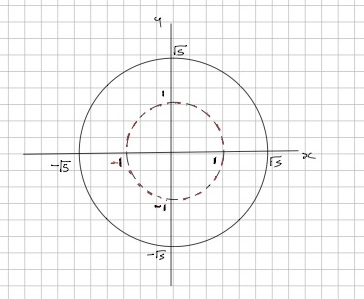
\includegraphics[scale=0.75]{question_8_A.jpg}\\
\vspace{1cm}
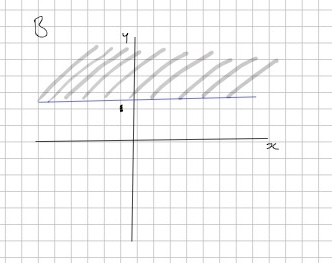
\includegraphics[scale=0.75]{question_8_B.jpg}\\
\vspace{1cm}
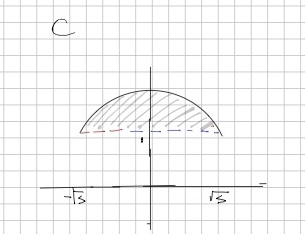
\includegraphics[scale=0.75]{question_8_C.jpg}


\vspace{5cm}

\qpart

\[ \left((0,1 + \frac{1}{n})\right)_{n=1}^{\infty} \]

By \textup{Definition 3.4 HB Chapter 13 p67},

The first component is a constant sequence \( \lim\limits_{n \to \infty} = 0 \) 
and constants sequences converge to the constant value.

The second component is \( 1 + \frac{1}{n} \).

\begin{align*}
\stext{Splitting this into two limits;}
\lim\limits_{n \to \infty} 1 = 1 \\[8pt]
\snote{Again it is a constant sequence, so it converges to \( 1 \).} \\[8pt]
\lim\limits_{n \to \infty} \frac{1}{n} = 0 \\[8pt]
\snote{As \( n \) approaches infinity, \( \frac{1}{n} \) approaches \( 0 \).} \\[8pt]
\stext{Combining these results;}
\lim\limits_{n \to \infty} (1 + \frac{1}{n}) = 1 + 0 = 1 \\[8pt]
\end{align*}

Therefore, by \textup{Definition 3.4 HB Chapter 13 p67}, the sequence
\[ \left((0,1 + \frac{1}{n})\right)_{n=1}^{\infty} \]
converges to
\[ \boxed{ (0,1) } \]

To test the limit point \( (0,1) \in A \),
\begin{align*}
1 < x^{2} + y^{2} &\leq 5 \\[8pt]
1 < 0^{2} + 1^{2} &\leq 5 \\[8pt]
1 < 1 &\leq 5 \\[8pt]
\stext{This is false, so \( (0,1) \notin A \)}
\end{align*}

To test the limit point \( (0,1) \in B \),
\begin{align*}
y &\geq 1 \\[8pt]
1 &\geq 1 \\[8pt]
\stext{This is true, so \( (0,1) \in B \)}
\end{align*}

Hence limit point \( (0,1) \notin A \) but \( (0,1) \in B \), 

Therefore \( (0,1) \notin C \).

\end{question}


%Question 10
\begin{question}

Question 10 from the TMA03 assignment.

Let
\[ R = (\Z, \oplus, \odot) \]
Where
\[ \oplus = a + b + 1 \]
and
\[ \odot = ab + a + b \]

\qpart
\begin{proof}
    $$ \newline

\textbf{R1 and R6 Closure of \( \oplus \) and \( \odot \);}
\begin{align*}
a, b, 1 &\in \Z \\[8pt]
\stext{Therefore,, because of closer under addition in \( \Z \),}
a + b + 1 &\in \Z \\[8pt]
\stext{So \( a \oplus b \in \Z \)} \\[8pt]
ab, a, b &\in \Z \\[8pt]
\stext{Therefore, because of closer under multiplication and addition in \( \Z \),}
ab + a + b &\in \Z \\[8pt]
\stext{So \( a \odot b \in \Z \)} \\[8pt]
\end{align*}

\textbf{R2 and R7 Associativity of \( \oplus \) and \( \odot \);}
\begin{align*}
\stext{For \( \oplus \),}
(a \oplus b) \oplus c &= (a + b + 1) + c + 1 \\[8pt]
&= a + b + c + 2 \\[8pt]
\stext{And}
a \oplus (b \oplus c) &= a + (b + c + 1) + 1 \\[8pt]
&= a + b + c + 2 \\[8pt]
\stext{So \( (a \oplus b) \oplus c = a \oplus (b \oplus c) \)} \\[8pt]
\stext{For \( \odot \),}
(a \odot b) \odot c &= (ab + a + b) \odot c \\[8pt]
&= (ab + a + b)c + (ab + a + b) + c \\[8pt]
&= abc + ac + bc + ab + a + b + c \\[8pt]
\stext{And}
a \odot (b \odot c) &= a \odot (bc + b + c) \\[8pt]
&= a(bc + b + c) + a + (bc + b + c) \\[8pt]
&= abc + ab + ac + a + bc + b + c \\[8pt]
\stext{So \( (a \odot b) \odot c = a \odot (b \odot c) \)} \\[8pt]
\end{align*}

\textbf{R3 Additive identity;}
\begin{align*}
\stext{Let \( e \) be the additive identity, then}
a \oplus e &= a \\[8pt]
a + e + 1 &= a \\[8pt]
e + 1 &= 0 \\[8pt]
e &= -1 \\[8pt]
\stext{So the additive identity is \( -1 \)} \\[8pt]
\end{align*}

\textbf{R8 Multiplicative identity;}
\begin{align*}
\stext{Let \( f \) be the multiplicative identity, then}
a \odot f &= a \\[8pt]
af + a + f &= a \\[8pt]
af + f &= 0 \\[8pt]
f(a + 1) &= 0 \\[8pt]
\stext{For a given \( a \) this can happen if  \( f = 0 \) or \( a = -1 \)} \\[8pt]
\stext{ But \( f \) must work for all \( a \), and we can choose \( a \neq -1 \) e.g. \( a = 0 \)} \\[8pt]
a + 1 &\neq 0 \\[8pt]
0 + 1 &\neq 0 \\[8pt]
1 &\neq 0 \\[8pt]
\stext{Hence \( f = 0 \)} \\[8pt]
\end{align*}

\textbf{R4 Additive inverse;}
\begin{align*}
\stext{Let \( g \) be the additive inverse of \( a \), then}
a \oplus g &= -1 \\[8pt]
a + g + 1 &= -1 \\[8pt]
g + a &= -2 \\[8pt]
g &= -a - 2 \\[8pt]
\stext{So the additive inverse of \( a \) is \( -a - 2 \)} \\[8pt]
\end{align*}

\textbf{R5 Commutativity of \( \oplus \);}
\begin{align*}
a \oplus b &= a + b + 1 \\[8pt]
&= b + a + 1 \\[8pt]
&= b \oplus a \\[8pt]
\stext{So \( a \oplus b = b \oplus a \)} \\[8pt]
\end{align*}

\textbf{R9 Distributive law;}
\begin{align*}
a \odot (b \oplus c) &= a \odot (b + c + 1) \\[8pt]
&= a(b + c + 1) + a + (b + c + 1) \\[8pt]
&= ab + ac + a + a + b + c + 1 \\[8pt]
&= ab + ac + 2a + b + c + 1 \\[8pt]
\stext{And}
(a \odot b) \oplus (a \odot c) &= (ab + a + b) \oplus (ac + a + c) \\[8pt]
&= (ab + a + b) + (ac + a + c) + 1 \\[8pt]
&= ab + ac + a + a + b + c + 1 \\[8pt]
&= ab + ac + 2a + b + c + 1 \\[8pt]
\stext{So \( a \odot (b \oplus c) = (a \odot b) \oplus (a \odot c) \)} \\[8pt]
\end{align*}

\textbf{R10 Commutativity of \( \odot \);}
\begin{align*}
a \odot b &= ab + a + b \\[8pt]
&= ba + b + a \\[8pt]
&= b \odot a \\[8pt]
\stext{So \( a \odot b = b \odot a \)} \\[8pt]
\end{align*}

Therefore, \( R \) is a commutative ring with identity.

\end{proof}

\vspace{5cm}

\qpart

By \textup{Definition 2.8 HB Chapter 12 p54}, we prove \( R \) is an integral domain;

\begin{proof}
    $$ \newline
From part a), we know \( R \) is a commutative ring with identity.

\textbf{No zero divisors;}
\begin{align*}
\stext{Let \( a, b \in R \) such that \( a \odot b = 0 \), then}
ab + a + b &= 0 \\[8pt]
\stext{adding 1 to both sides,}
ab + a + b + 1 &= 1 \\[8pt]
\stext{Factorising the LHS,}
(a + 1)(b + 1) &= 1 \\[8pt]
\stext{Since \( a, b \in \Z \), the only way for the product to be 1 is if both \( (a + 1) = 1 \) and \( (b + 1) = 1 \)} \\[8pt]
a + 1 &= 1 \\[8pt]
b + 1 &= 1 \\[8pt]
\stext{Therefore,} \\
a &= 0 \\[8pt]
b &= 0 \\[8pt]
\stext{So the only way for \( a \odot b = 0 \) is if \( a = 0 \) or \( b = 0 \)} \\[8pt]
\end{align*}
Therefore, \( R \) has no zero divisors, and is an integral domain.
\end{proof}

\vspace{3cm}

\qpart

By \textup{Definition 1.14 HB Chapter 11 pg48}, we have already shown \textbf{R1-R10}, so we also need 
to find a multiplicative inverse for every non-zero element in \( R \).

\textbf{Multiplicative inverse;}

\begin{align*}
\stext{Let \( a \in R \) and \( a \neq 0 \), and let \( h \) be the multiplicative inverse of \( a \), then}        
a \odot h &= 0 \\[8pt]
ah + a + h &= 0 \\[8pt]
ah + h &= -a \\[8pt]
h(a + 1) &= -a \\[8pt]
h &= \frac{-a}{a + 1} \\[8pt]
\stext{So the multiplicative inverse of \( a \) is \( \frac{-a}{a + 1} \)} \\[8pt]
\stext{However, for \( h \) to be in \( R \), \( \frac{-a}{a + 1} \) must be an integer, which is not the case for all \( a \in R \)} \\[8pt]
\stext{For example, if \( a = 1 \), then \( h = \frac{-1}{2} \notin \Z \)} \\[8pt]
\end{align*}

Therefore, not every non-zero element in \( R \) has a multiplicative inverse, and so \( R \) is not a field.

\end{question}

\end{document}